\subsection{Setzeinheit}
\textit{(ygu)} Die Setzeinheit bezeichnet alle Teile, welche durch die Translation bewegt werden. Auch zur Setzeinheit gehören die Spindel sowie der Spindelantrieb, welche die Translation umsetzen.
\newline
Die wesentlichen Komponenten der Setzeinheit sind in Abbildung \ref{fig:setzeinheit} dargestellt. Dabei wird in diesem Unterkapitel ausschliesslich auf die Komponenten der Setzeinheit eingegangen. Alle Komponenten die zur Verstellung des Topfradius dienen, sind in der Abb.  \ref{fig:setzeinheit} unter Punkt 6 (Verstellmechanik) gesammelt und werden im Kapitel \ref{verstellmechanik} näher erläutert.
\newline
\newline
\textbf{Aufbau}
\newline
Die Spindel ist durch eine bewegte Montageplatte (Punkt. 15 in Abb. \ref{fig:setzeinheit}) und drei Führungen (5) mit der Verstellmechanik (7) verbunden. Diese Führungen werden durch drei Gleitlager (6)  an einer Montageplatte (13) gelagert. die zwei oberen Montageplatten (11, 12) dienen zur Montage des Spindelantriebes sowie zur Lagerung der Spindel (4). Um eine weitere Montageplatte zu sparen, ist der Spindelantrieb mittels einer Distanzhülse (2) mit der obersten Montageplatte (11) verbunden. Die unterste Montageplatte (14) dient zur Lagerung der Verstellmechanik sowie zum einfachen Schutz der Mechanik vor Topferde. Dadurch ist gewährleistet das nur ein minimaler Teil (der Stechdorn, 8) der bewegten Komponenten in Kontakt mit der Topferde kommt.
	\begin{figure}[H]
	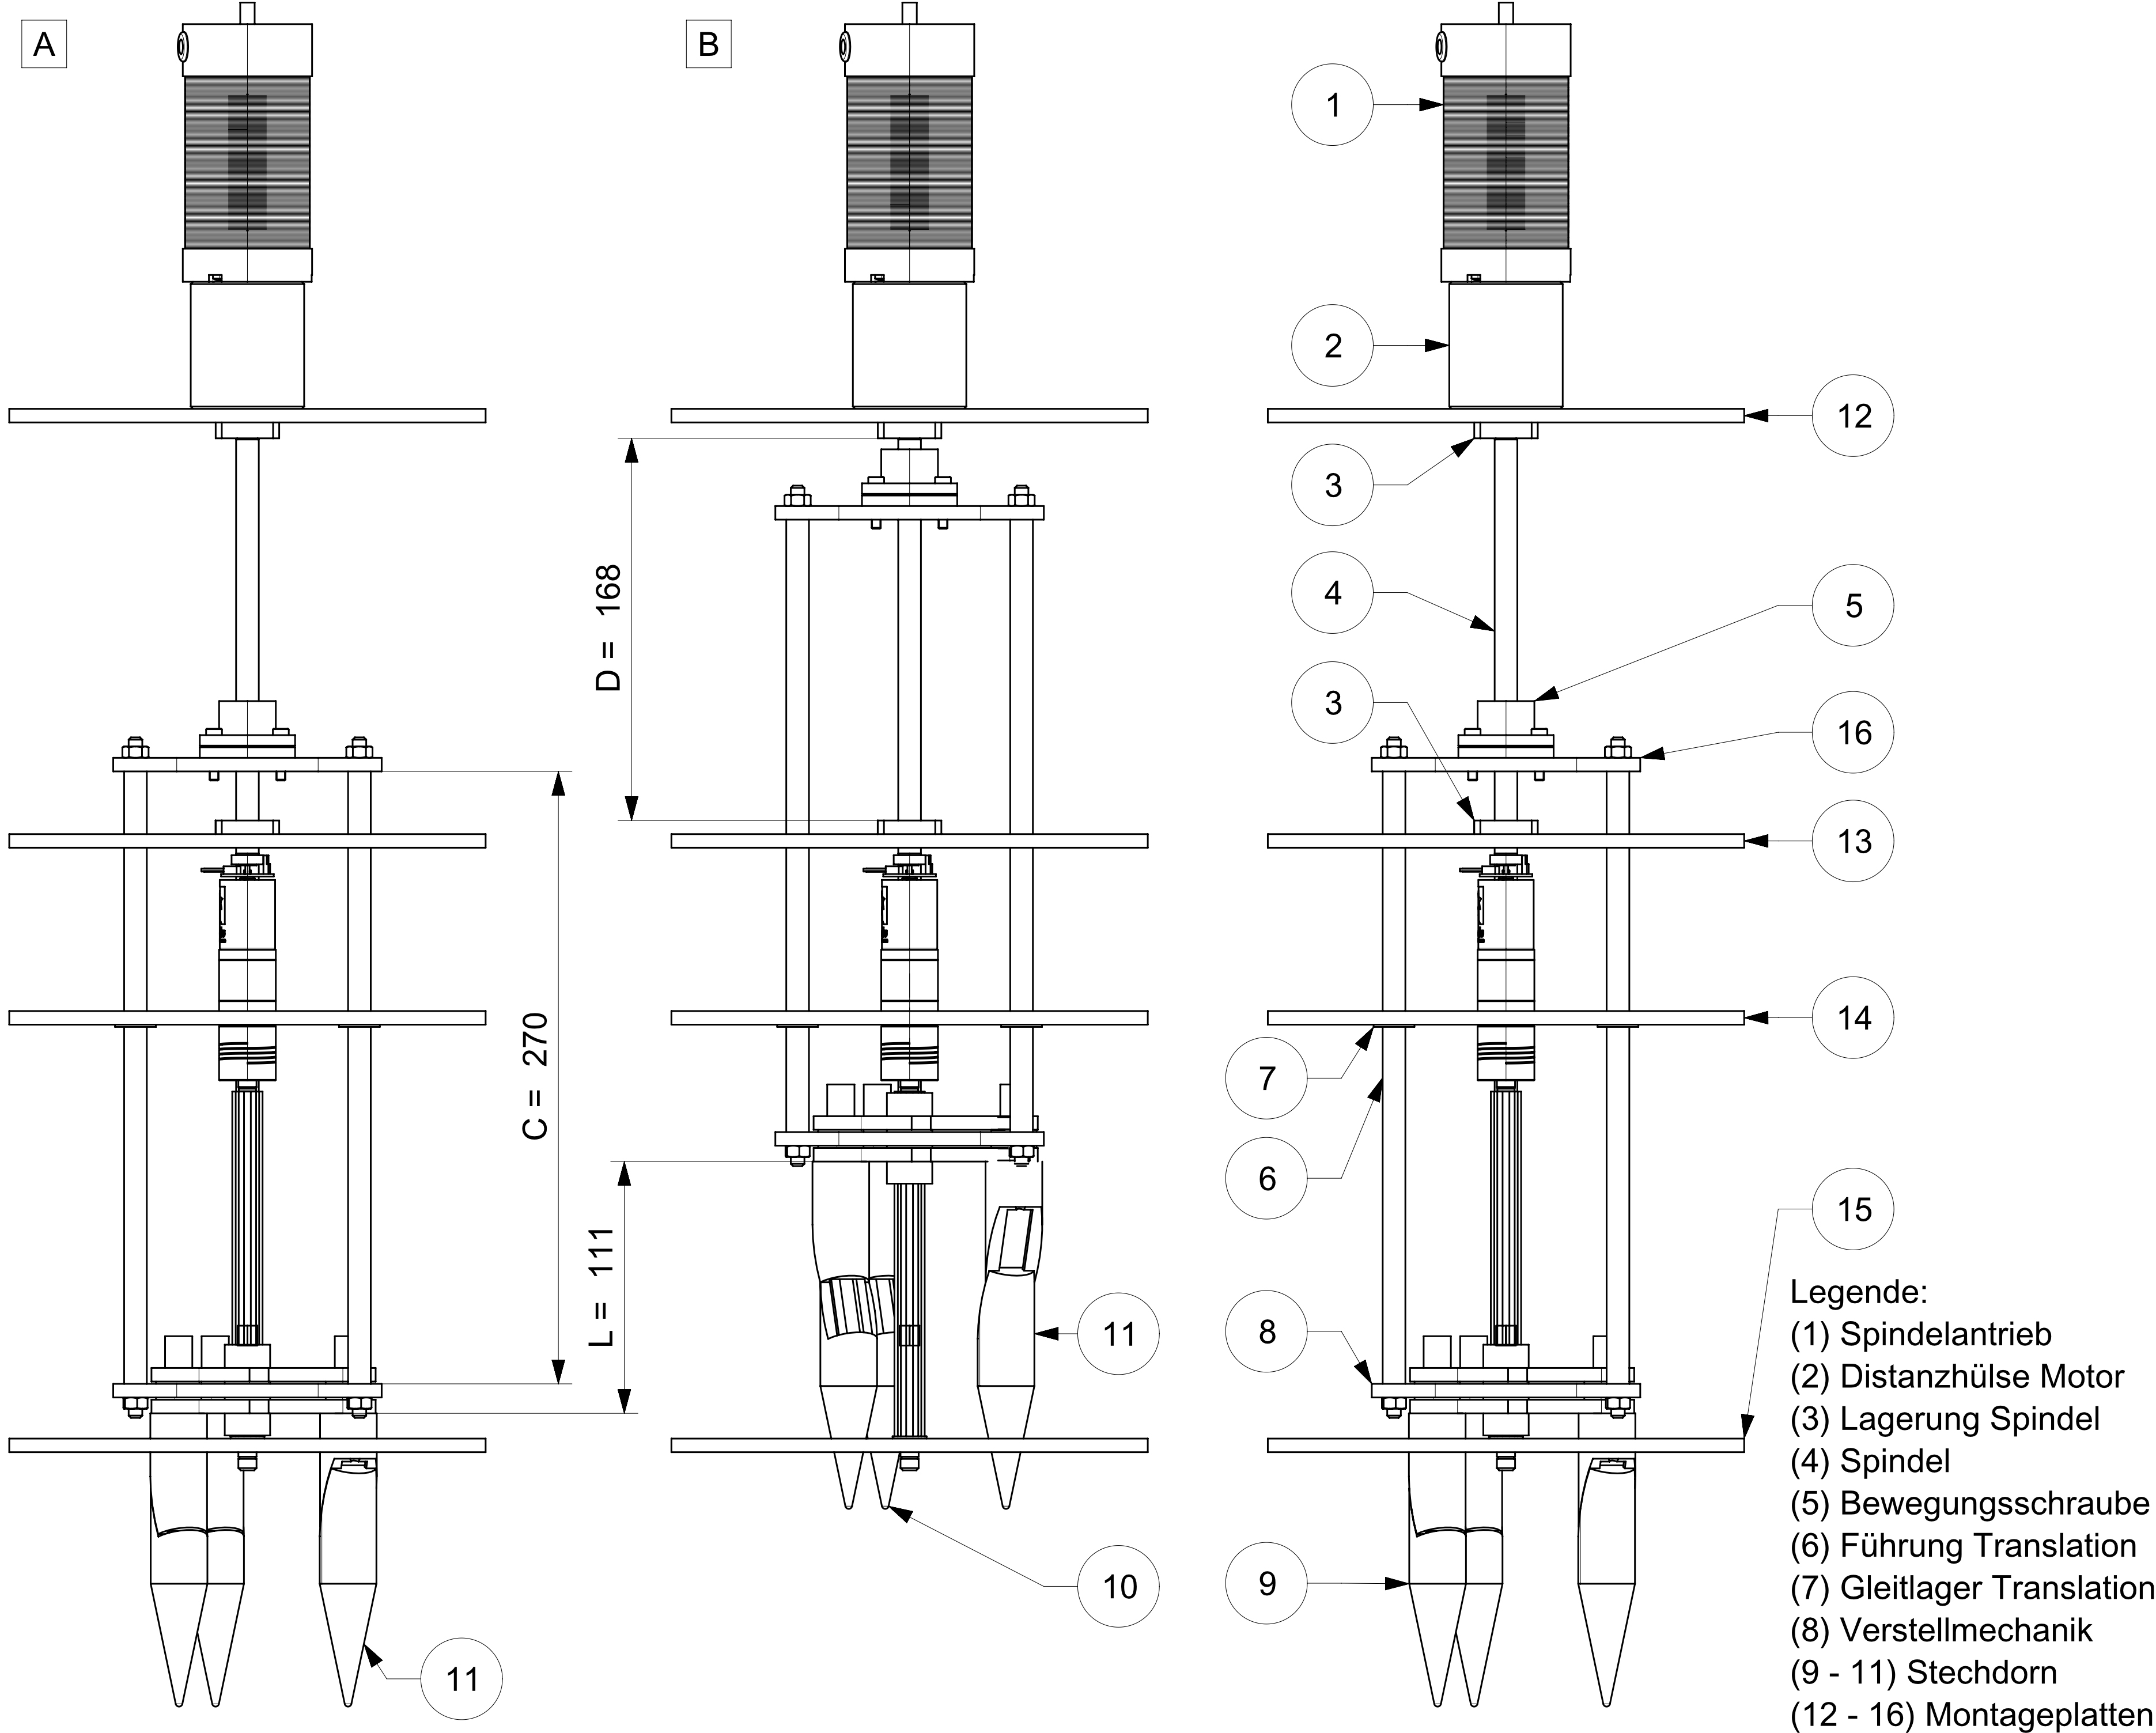
\includegraphics[scale=0.53]{Illustrationen/6-Umsetzung/setzeinheit_aio.jpg}
	\caption{Detaillierte Übersicht der Setzeinheit}
	\label{fig:setzeinheit}
\end{figure}

 
\subsubsection{Translation der Setzeinheit}
Die Setzeinheit macht folgenden Bewegungsablauf, um drei NemaCaps in einen Topf zu pflanzen:
\begin{itemize}
	\item \textbf{A - Setzloch ausheben:} Die Spindel bewegt die Setzeinheit nach unten und treibt den Stechdorn in die Erde. Dadurch verschliesst sich der Stechdorn (Punkt 9 in Abb. \ref{fig:setzeinheit}). 

	\item \textbf{B - NemaCap setzen:} Nachdem die Erde verdrängt und das Setzloch ausgehoben ist, bewegt sich die Setzeinheit wieder nach oben. Nun öffnet sich der Stechdorn (10) indem sich der untere Teil durch die Schwerkraft auf die Seite bewegt. So können die NemaCaps in das ausgehobene Setzloch fallen.
\end{itemize}

Konstruktiv sind drei Masse hervor zu heben:
\begin{itemize}
	\item \textbf{L - Maximaler Hubweg:} Der maximale Hub L beträgt 111mm. Gemäss Berechnungen (\textbf{Siehe Anhang XY}) muss dieser mindestens 86mm betragen. Somit beträgt die Reserve 25mm. 
	
	\item \textbf{C - Länge der Führungen:} Die Länge der Führungen ist gegeben durch den Hubweg L, die Höhe des Motors für die Verstellmechanik dessen Kupplung. Dies bedingt eine Länge von 270mm.
	
	\item \textbf{D - Länge der Spindel:} Die Spindellänge ist gegeben durch den maximalen Hub L, der Höhe der Bewegungsschraube sowie die Montageplatte.
\end{itemize}
\textbf{Lagerung}
\newline
Die Lagerung der translatorischen Bewegung wird durch drei Gleitlager (Punkt. 6 in Abb. \ref{fig:setzeinheit}) realisiert. Dabei werden diese in die Montageplatte (12) eingepresst. Dafür werden drei Kunststoff Gleitlager iglidur J3FM-1012 von igus verwendet. Begründet wird die Wahl dadurch, dass Kunstoffgleitlager schmiermittel- und wartungsfrei sind, geringe Reibwerte und eine hohe Lebensdauer aufweisen. Weiter sind dies Standard-Maschinenelemente und dadurch günstig erhätlich. Weitere Informationen die Gleitlager sind aus dem Datenblatt zu entnehmen.
\newline
\textbf{Kinetik?}
\newline
\textbf{Knickgefahr?}
\newline

\subsubsection{Spindel}
Die Wahl der Spindel und des Spindelantriebes haben einen entscheidenden Einfluss auf die Erfüllung des Setzprozesses innerhalb der vorgegeben Zeit. Parameter wie Steigung, Spindeldurchmesser und Material der Spindel wirken sich direkt auf die Massenträgheit und somit auf das erforderliche Beschleunigungsmoment aus.
 \\
 \newline
\textbf{Auslegung und Wahl}
 \\
Die Subkapitel befasst sich mit der Auslegung und Berechnung der Spindel. Dabei sind Berechnungen in zusammengefasster Form dargestellt. Der vollständige Rechenweg und die detailierte Vorgehensweise sind im Anhang (\textbf{Datei XY}) zu entnehmen.

Gegeben durch den Setzprozess und die Geometrie sind folgende Daten:
	\begin{figure}[H]
	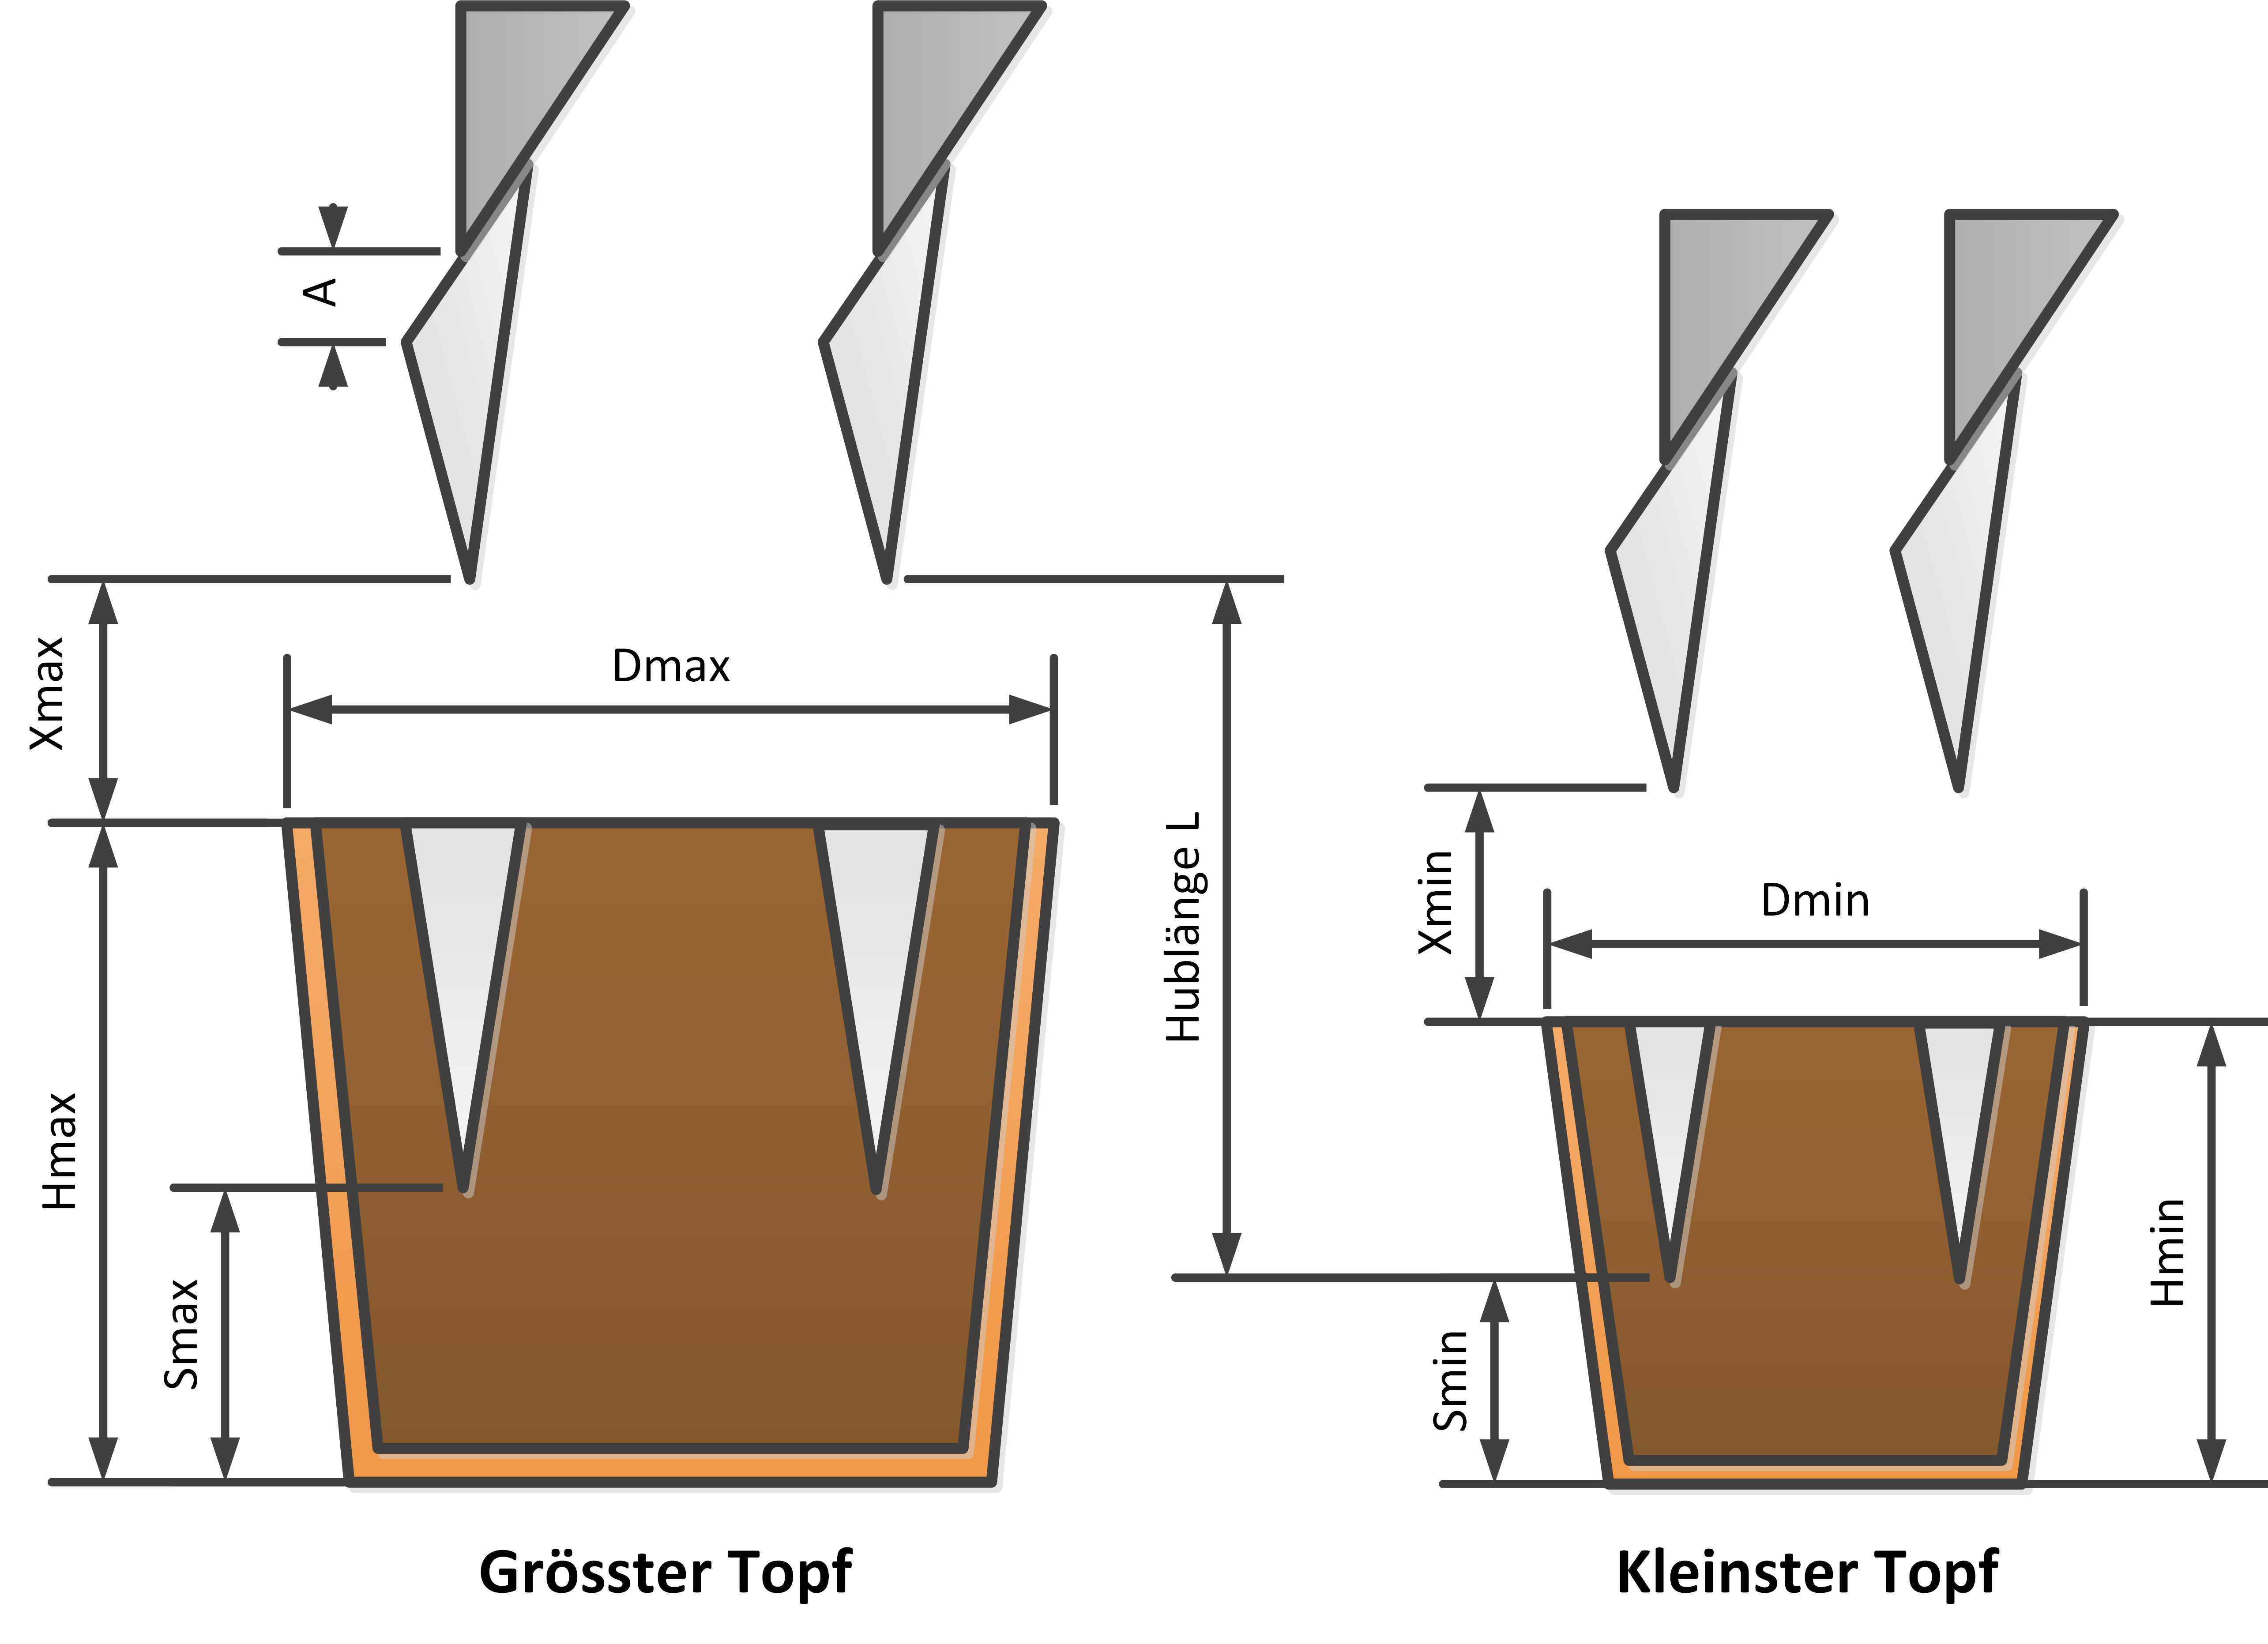
\includegraphics[width=1\textwidth]{Illustrationen/6-Umsetzung/topfgeometrie.png}
	\caption{Geometrie der Töpfe und des Setzprozess}
	\label{fig:topfgeometrie}
	\end{figure}
\begin{table}[H]
\begin{tabular}{|l|c|c|l|}
	\hline 
	& Grösster Topf (max) & Kleinster Topf (min) & Kommentar \\ 
	\hline 
	Durchmesser D [mm] & 140 & 90 & Aus Datenblatt \\ 
	\hline 
	Höhe h [mm] & 106 & 67 & Aus Datenblatt \\ 
	\hline 
	max. Einsetztiefe S [mm] & 63.6 & 40.2 & 0.6 x Höhe \\ 
	\hline 
	Sicherheitsabstand X [mm] & 15 & 15 & Annahme \\ 
	\hline 
	Ausfahrlänge A Dorn [mm] & 15 & 15 & Annahme \\ 
	\hline 
\end{tabular} 
	\caption{Randbedingungen für Spindelauslegung}
	\label{tab:Randbedingungen}
\end{table}

Anhand dieser Randbedingungen und den getroffenen Annahmen ergibt sich eine Beschleunigungs- und Bremszeit tb=0.1125s. Bei einem maximalen Hubweg Umax = 72.4mm beträgt die grösste durschnittliche Geschwindigkeit vavmax:

\begin{equation}
v_{avmax}=\frac{U_{max}}{t_{b}}=\frac{72.4mm}{0.1125s}=643.5mm/s
\end{equation}
\newline
Die Geschwindigkeit des Dornes kann streng idealisiert gemäss Abbildung \ref{fig:vprofil_dorn} dargestellt werden:
	\begin{figure}[H]
	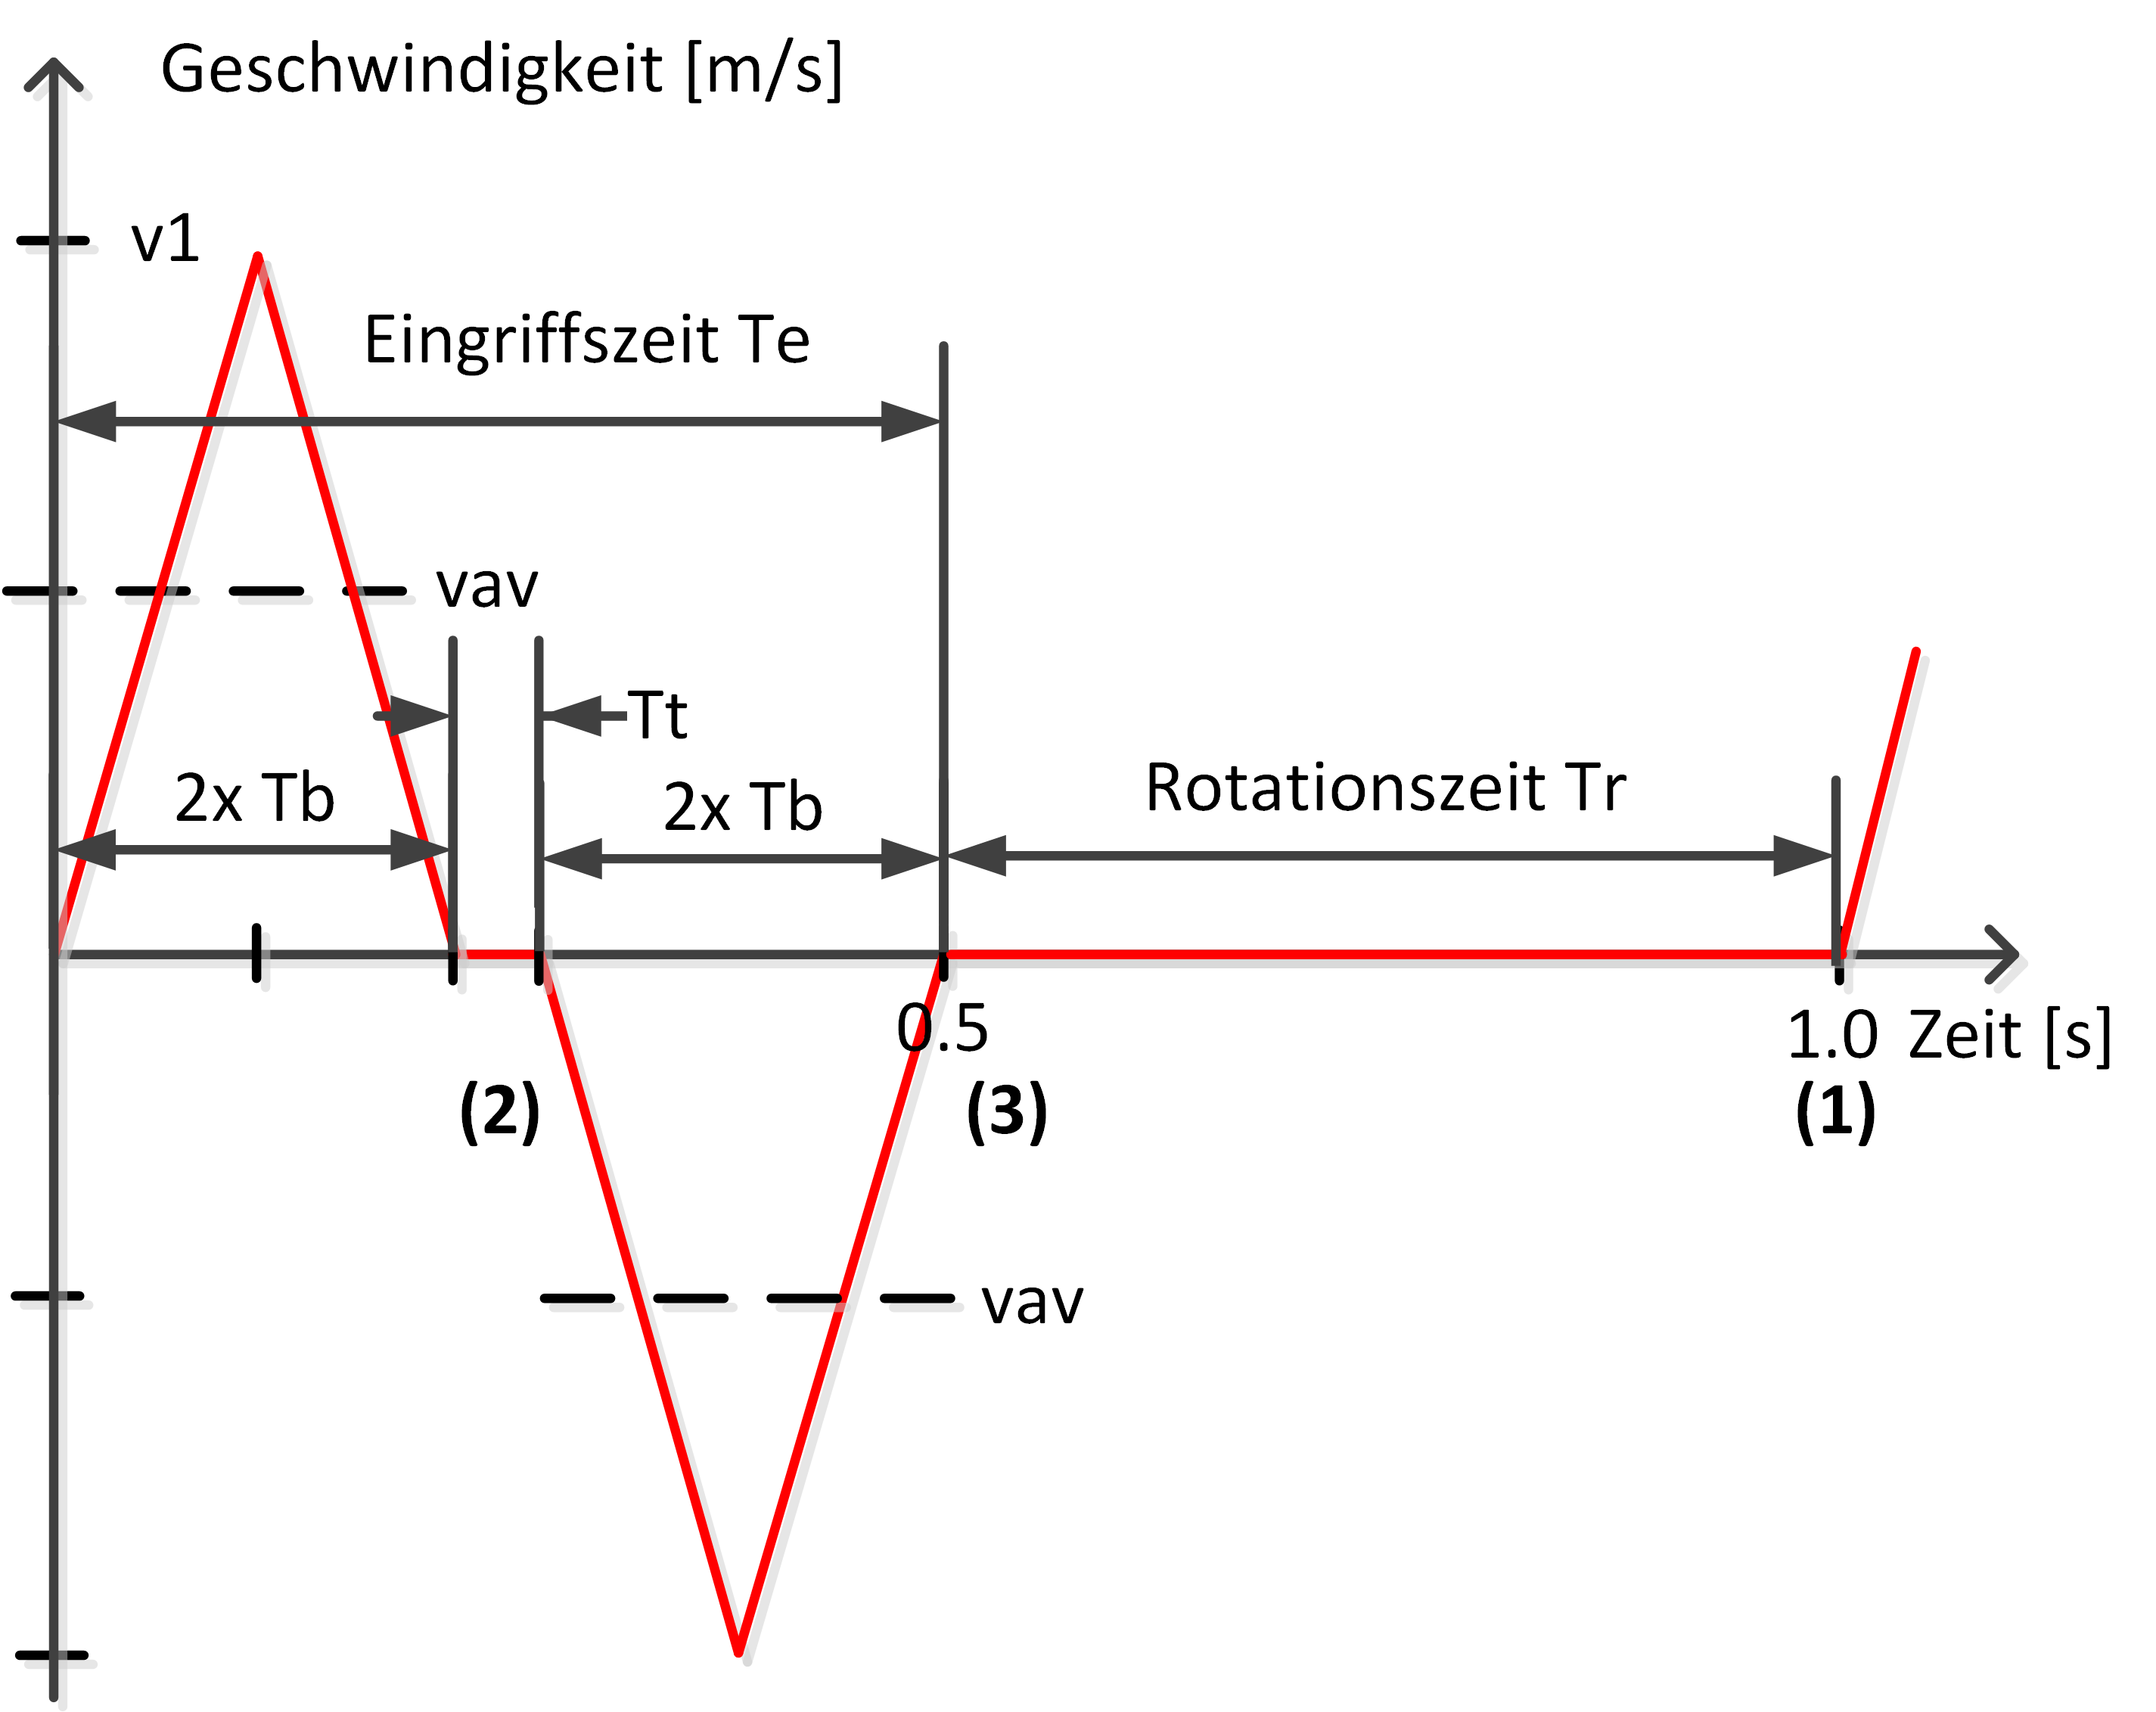
\includegraphics[width=1\textwidth]{Illustrationen/6-Umsetzung/vprofil_dorn.png}
	\caption{Geschwindigkeitsprofil des Dorns}
	\label{fig:vprofil_dorn}
\end{figure}
Orientiert an den Anforderungen aus Kapitel \ref{subsec:Translation} und der berechneten Geschwindigkeit sind vier Steilgewindespindeln von Igus ausgewählt worden. In Rücksprache mit Mark Chalençon, Produktmanager bei igus Schweiz GmbH, wurde die Auswahl der Produkte zusätzlich verifiziert (Mail vom 18.4.17).
\begin{table}[H]
\begin{tabular}{|c|c|}
	\hline 
	Ds14x30 (Edelstahl) & Ds10x25 (Edelstahl) \\ 
	\hline 
	Ds14x30 (Aluminium) & Ds10x25 (Aluminium) \\ 
	\hline 
\end{tabular} 
\caption{Ausgewählte Steilgewindespindeln von Igus}
\label{tab:spindeln}
\end{table}
Mit diesen Angaben kann die Spindel durch ein reduziertes Model dargestellt werden, analog zu Abbildung 13-5, S.448 \cite{roloffmatek}:
 	\begin{figure}[H]
 	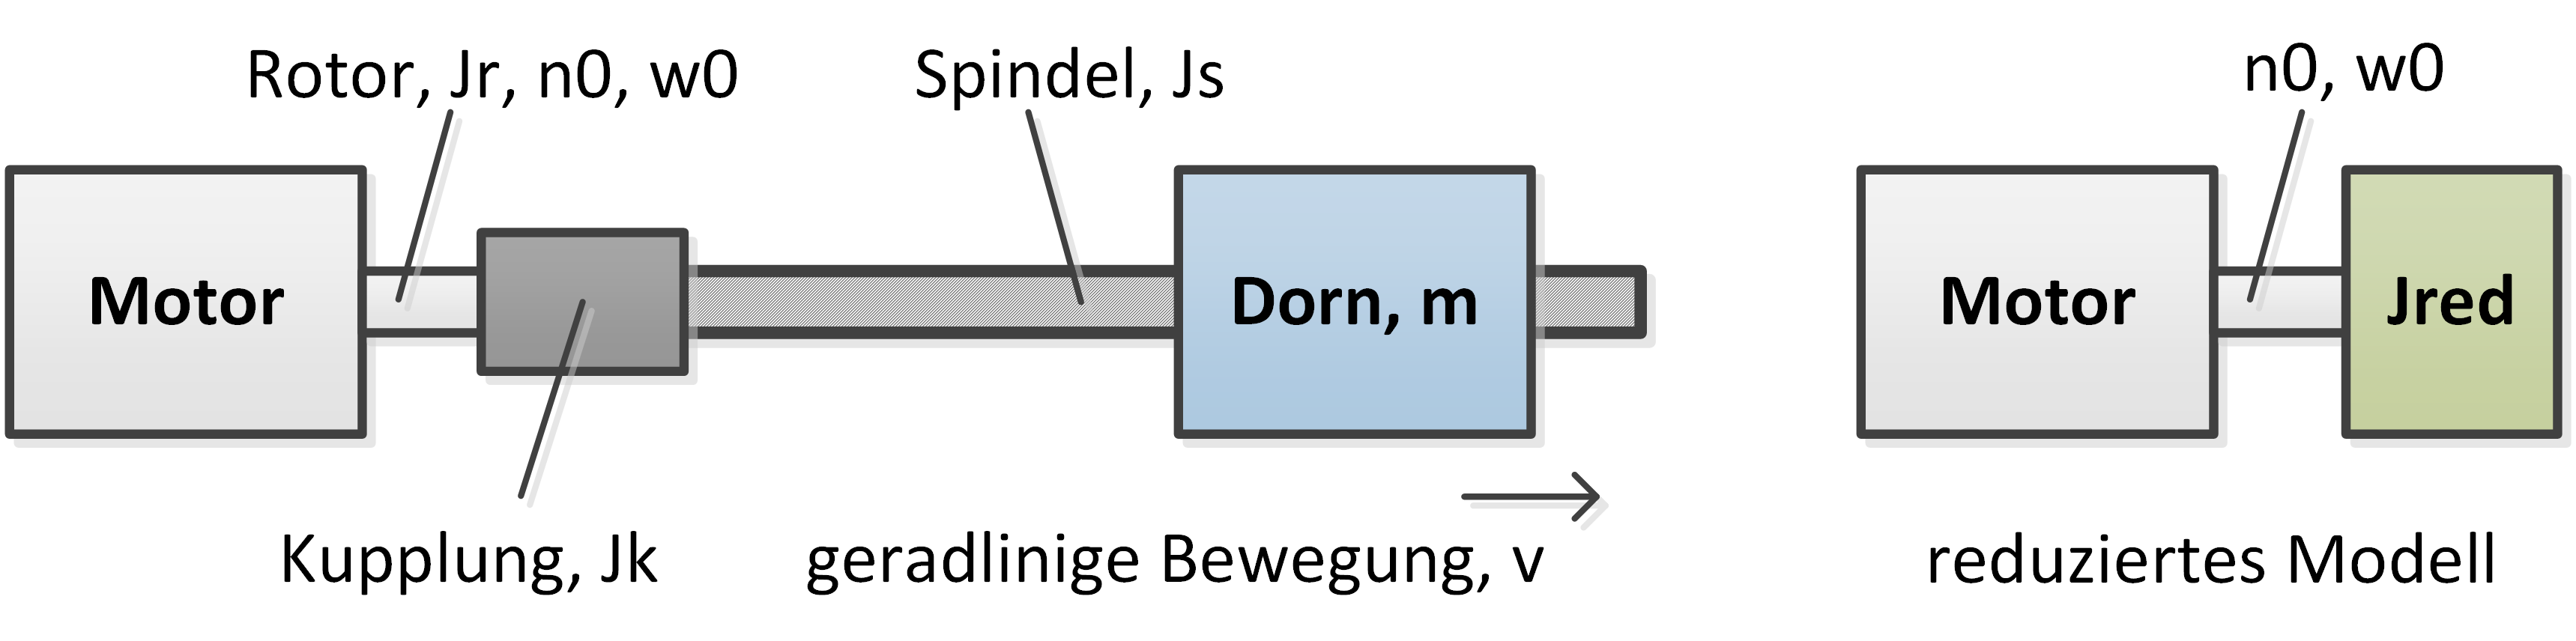
\includegraphics[width=1\textwidth]{Illustrationen/6-Umsetzung/red_modell.png}
 	\caption{Schema des Spindelantriebs sowie des reduzierten Modells}
 	\label{fig:red_modell}
	\end{figure}
wobei für das reduzierte Modell sich die reduzierte Massenträgheit Jred und das benötigte Beschleunigungsmoment Ma ergibt (Gleichung 13.3 und 13.4, S.449):
\begin{equation}
J_{red}=J_{rotor}+J_{kupplung}+J_{spindel}+m*(\frac{v_{1}}{w_{v1}})^{2}
\end{equation}
\begin{equation}
M_{a}=J_{red}*\frac{w_{2}-w_{1}}{t_{b}}=J_{red}*\frac{w_{v1}}{t_{b}}
\end{equation}
Für die ausgewählten Spindeltypen ergibt dies folgende Werte:
\newline
\textbf{Tabelle der Spindeln}
Die berechneten Werte für das Beschleunigungsmoment Ma aus \textbf{Tabelle XY} zeigen, dass sich alle ausgewählten Spindeln für den evaluierten Spindelantrieb eignen.
\newline
\newline

Als definitive Wahl wird die Spindel Ds10x25 aus Edelstahl ausgewählt. Folgende Argumente sind ausschlaggebend:
	\begin{itemize}
	\item Die Variante Ds10x25 aus Edelstahl bietet das Optimum von geringem Durchmesser und hoher Festigkeit. Das leicht höhere Beschleunigungsmoment der Ds10x25 aus Edelstahl zur Ds14x30 wird für eine höhere Festigkeit in Kauf genommen.
	
	\item \ Die geringere Steigung gibt dem Motor mehr Weg (Umdrehungen) zur Beschleunigung.
\end{itemize}
\textbf{Lagerung und Kupplung der Spindel}
\newline
Die Spindel wird durch ein Fest- sowie ein Loslager eindeutig gelagert. Das Festlager ist in der obersten Montageplatte (Punkt. 11 in Abb. \ref{fig:setzeinheit}) vorgesehen, das Loslager in der zweiten Montageplatte (12). Diese Anordnung ist bewusst so gewählt, sodass das Festlager Axialkräfte aufnimmt und Spindelantrieb axial unbelastet bleibt. Für die Lagerung werden fertige Lagerböcke von Mädler Norm-Antrieb AG verwendet, welche speziell für Spindeln ausgelegt sind. Diese sind einfach im Einbau und erfordern keinen zusätzlichen Entwicklungsaufwand. An der Spindel wird konstruktiv einen Freistich Form E gemäss Normen-Auszug umgesetzt (\textbf{Siehe Zeichnung XY})\cite{vsm}.
\newline
Zur mechanischen Verbindung zwischen Spindelantrieb und Spindel wird eine drehstarre Kupplung verwendet. Dadurch kann eine winkelgetreue Drehmomentenübertragung gewährleistet werden, was für diese Anwendung essentiell ist. Hierfür wird die Kupplung HELICAL WA 20-8-6 aus Aluminium von Ringspann AG verwendet. Die Wahl eines kleinen Aussendurchmessers (20mm) und eine leichter Werkstoff sind für ein möglichst geringes zusätzliches Trägheitsmoment entscheidend und wurde hier berücksichtigt.
\subsubsection{Montage}
Wie schon mehrfach erwähnt werden mehrere verschiedenste Komponenten an Montageplatten montiert. Wie aus Abbildung \ref{fig:setzeinheit} ersichtlich, werden die Montageplatten vertikal angeordnet. Diese Anordnung bildet so das Gerüst für eine funktionierende Setzeinheit. Wie in Kapitel XY erwähnt, bietet sich die konsequente Fertigung mittels Lasermaschine an. Mechanisch fixiert werden die Montageplatten durch Aluminium Profile der Firma Kanya AG (weitere Informationen in \textbf{Kap XY}), wobei durch die Nut der Profile eine Blechdicke von 6mm vorgegeben ist. Diese Konstruktion bringt folgende Vorteile:
	\begin{itemize}
	\item Auf unterschiedlichen Ebenen können so Komponenten angeordnet werden. Das Hinzufügen von weiteren Komponenten ist auf einfachste Art realisierbar. Kommt eine Komponente hinzu, wird die benötigte Kontur (z.B. ein Langloch oder Bohrung) vorgesehen und die Komponente ist montierbar.
	\item Die Fixierung der Montageplatten durch Aluminium-Profile bringt weitere Flexibilität bei der Montage. Dadurch bleibt die Höhe der einzelnen Platten verstellbar. Auch seitlich können die Platten in eine Richtung verstellt werden.
\end{itemize}
 	\begin{figure}[H]
	\includegraphics[width=1\textwidth]{Illustrationen/6-Umsetzung/Montageplatten.png}
	\caption{Übersicht der Montageplatten}
	\label{fig:montageplatten}
\end{figure}
Die Montageplatten 1 bis 3 aus Abbildung \ref{fig:montageplatten} verfügen über drei Langlöcher (Detail A), welche um jeweils 120° verschoben angeordnet sind. Diese sind für die flexible Führung der Schläuche vorgesehen.